\documentclass[12pt,a4paper]{article}
\usepackage{longtable}
\usepackage[LGR,T1]{fontenc}
\usepackage{lscape}
%\usepackage{pdfsync}
\usepackage{multirow}
\usepackage{amsmath,bm} 
\usepackage{amsfonts}
\usepackage{amsthm} % Extended theorem environments
%\usepackage{amssymb} % Math symbols %%redundant with stix package
%\usepackage{esint} % Intégrales multiples
%\usepackage{esvect} % Vecteurs
\usepackage{mathtools}
\usepackage{pifont} 
 
\usepackage{fancyhdr}
\usepackage{graphicx}

\graphicspath{{../frontend/img/}{../chap_intro_ccl/img/}{../chap_case_study/img/}{../chap_ES_PCE/img/}{../chap_electro_uq/img/}{../chap_methodo/img/}{../chap_myopic/img/}{../chap_RL/img/}{../chap_atom_mol/img/}{../chap_RobPol/img/}{../appendices/img/}} % Figures folder different for each input
%\graphicspath{{img/}} %
\DeclareGraphicsExtensions{.eps,.pdf,.png,.jpg}




\usepackage{lastpage}
\usepackage{afterpage}
\usepackage{lettrine}
\usepackage{color,soul}
\usepackage[dvipsnames]{xcolor}
\usepackage{colortbl}
\usepackage{enumitem}
\usepackage{tikz}
\usepackage{titlesec}
\def\eg{e.g.,\ }
\def\ie{i.e.,\ }


%Palatino font
%\usepackage{pxfonts}
%\usepackage{libertine}
\usepackage[scaled=0.88]{beraserif}
\usepackage[scaled=0.85]{berasans}
\usepackage[scaled=0.84]{beramono}
\usepackage{mathpazo}
%\linespread{1.05}
\usepackage[T1,small,euler-digits]{eulervm}

\usepackage[nomessages]{fp}


\definecolor{bleuUCLclair}{rgb}{.09, 0.569, 1}
\definecolor{bleuUCLfonce}{rgb}{ .13, .52, .86}
\definecolor{redBurn}{rgb}{.91, 0.29, 0.08}

\usepackage{tocloft}
\renewcommand{\cftsecpresnum}{Reviewer \#}
\renewcommand{\cftsecnumwidth}{6em}
\renewcommand{\cftsubsecpresnum}{Comment \#}
\renewcommand{\cftsubsecnumwidth}{6em}

\usepackage[colorlinks=true,urlcolor=black,linkcolor=black,citecolor=black]{hyperref}
\usepackage[square,numbers,sort&compress]{natbib}

\bibliographystyle{biblio/elsarticle-num-names}  %Ordered by appearance in the text, with DOI and URL
%\usepackage[backend=biber, natbib=true, style=numeric-comp, citestyle=numeric-comp, sorting=none, giveninits=true, maxcitenames=1]{biblatex}

\usepackage[]{tocbibind}
\usepackage{hyperref}
\hypersetup{
    colorlinks=true,
%    linkcolor=black,
    bookmarks=true,
    pdfpagemode=FullScreen,
}
\setcounter{tocdepth}{1}

\addtolength{\topmargin}{-1.5cm}
\addtolength{\textheight}{1.5cm}
\addtolength{\textwidth}{2cm}
\addtolength{\footskip}{2cm}
\setlength{\evensidemargin}{-0.5cm}
\setlength{\oddsidemargin}{-0.5cm}
\setlength{\arrayrulewidth}{0.25pt}

\renewcommand{\baselinestretch}{1.1} % Interligne


\newenvironment{maliste}%
{ \begin{list}%
	{\textcolor{bleuUCLfonce}{$\bullet$}\hspace{0.5cm}}%
	{\setlength{\labelwidth}{50pt}%
	 \setlength{\leftmargin}{25pt}%
	 \setlength{\itemsep}{30pt}}}%
{ \end{list} }

%\renewcommand{\headrulewidth}{0.0pt}
%\newcommand{\clearemptydoublepage}{%
%	\newpage{\pagestyle{empty}\cleardoublepage}}




%section like title in longtable
\newcommand{\seclong}[1]{\multicolumn{2}{@{}l}{{\Large\sffamily #1}} 
\vspace{0.5cm}
\\}

%enumerate on two columns
\newcounter{listlong}
\newcommand{\newlistlong}{\setcounter{listlong}{1}}
\newcommand{\iteml}[1]{%
\hspace{4.5cm}\textcolor{redBurn}{\arabic{listlong}}\stepcounter{listlong}%
&%
#1%
 
\\%
}

%left in column
\newcommand{\lcol}[1]{%
\begin{minipage}[t]{.35\textwidth}%

#1%

\end{minipage}%
}

\title{\vspace{-1cm}
\begin{flushleft} {\sffamily Xavier Rixhon's PhD thesis - Answers to jury members}\end{flushleft}}
\date{\vspace{-1.7cm}\begin{flushleft}\sffamily Exploration of uncertainty-aware energy transition pathways - Reinforcement learning and principal component analysis-based methods\end{flushleft}}
%
%Xavier Rixhon, Gauthier Limpens, Diederik Coppitters, Hervé Jeanmart and Francesco Contino\end{flushleft}}


\pagestyle{fancy} 
\fancyhf{}
\fancyfoot[R]{\sffamily\thepage\ / \pageref{LastPage}}
  \fancyfoot[L]{ }

\fancypagestyle{plain}{%
  \fancyhf{}%
  \fancyfoot[R]{\sffamily\thepage\ / \pageref{LastPage}}
  \fancyfoot[L]{ }
}

\renewcommand{\headrulewidth}{0.0pt}


\newcommand{\hlc}[2][yellow]{ {\sethlcolor{#1} \hl{#2}} }

\titleformat{\section}
  {\bfseries\scshape}{}{1em}{}

\titleformat{\subsection}
  {\normalfont\scshape}{}{1em}{}

\usepackage[framemethod=default]{mdframed}
%\mdfsetup{skipabove=\topskip,skipbelow=\topskip}

\global\mdfdefinestyle{comment}{%
     linecolor=red,linewidth=0.1cm,%
     leftmargin=-0.5cm,rightmargin=-0.5cm, innerleftmargin=0.4cm,innerrightmargin=0.4cm,
     topline=false,bottomline=false
}

\global\mdfdefinestyle{manuscript}{%
     linecolor=gray!20,linewidth=0.05cm,backgroundcolor=gray!20,%
     leftmargin=-0.5cm,rightmargin=-0.5cm, innerleftmargin=0.4cm,innerrightmargin=0.4cm
}
  
  \renewcommand{\subsectionautorefname}{Comment}
\begin{document}
\maketitle
%\emph{Start with some thank you note. For example:}

I would like to thank the jury members for the comments, which significantly helped improving the manuscript and substantiating the novelty of my work. Based on the notes taken during the private defense, I hereby transcribed, as accurately as possible, the jury's comments. 

I believe I have addressed all the issues raised in the following answers. Some of them required adaptations of the text. These adaptations are either directly in the thesis manuscript or left for further developments in subsequent papers. For each comment, I have first highlighted the issue, then provided an answer, and finally described how the manuscript was adjusted, if needed.\\

When a comment explicitly came from specific members of the jury, they are listed at the beginning of the comment with the following color code: {\color{orange} \textbf{Stefano} Moret}, {\color{teal} \textbf{Stefan} Pfenninger}, {\color{purple} \textbf{Sylvain} Quoilin} and {\color{violet} \textbf{Christophe} De Vleeschouwer}. Here is how an answer to a comment is structured:

\begin{mdframed}[style=comment] % Comment from the reviewer
Text of the comment.
\end{mdframed}

\noindent The answer provided to the comment and, based on this, where the potential modification brought to the manuscript is located in the thesis manuscript using {\color{blue} blue font}.

\begin{mdframed}[style=manuscript] % Modification brought to the manuscript
New version of the text in the manuscript.
\end{mdframed}

% {\color{orange} \textbf{Stefano}}
% {\color{purple} \textbf{Sylvain}}
% {\color{teal} \textbf{Stefan}}
% {\color{violet} \textbf{Christophe}}

\clearpage

\section{General comments/questions}
\label{General}

\begin{mdframed}[style=comment] % Comment from the reviewer
{\color{orange} \textbf{Stefano}} - Overall, many methods: PCE + RL + NN + PCA. At each stage, some assumption is made. Why not a simpler approach or a simpler model? Do you need all these steps? 
\end{mdframed}

\noindent

\begin{mdframed}[style=manuscript] % Comment from the reviewer

\end{mdframed}

\subsection{Assumptions - Fine tuning}
\label{fine_tuning}

\begin{mdframed}[style=comment] % Comment from the reviewer
{\color{orange} \textbf{Stefano}} - Many assumptions, e.g., alpha = 85\% (p. 40) or reward = -300 (Chapter 4). How sensitive are the results to these assumptions? It looks like all these parameters have been tuned to obtain the desired results. How robust are they?
\end{mdframed}

\noindent

\begin{mdframed}[style=manuscript] % Comment from the reviewer

\end{mdframed}

\subsection{Graphs}
\label{general_graphs}

\begin{mdframed}[style=comment] % Comment from the reviewer
{\color{orange} \textbf{Stefano}} \& {\color{teal} \textbf{Stefan}} - Graphs should be better explained. Many axes labels are missing, and the captions are often insufficient to read the figures. 
\end{mdframed}

\noindent

\begin{mdframed}[style=manuscript] % Comment from the reviewer

\end{mdframed}

\subsection{Structure}
\label{structure}

\begin{mdframed}[style=comment] % Comment from the reviewer
{\color{orange} \textbf{Stefano}} - The thesis structure makes it quite difficult to follow. Having all the methodology summarised in Chapter 1, makes it difficult to link it to the different chapters. As changing the structure may be now a major work, I would invite you to think how to better connect the different parts. 
\end{mdframed}

\noindent

\begin{mdframed}[style=manuscript] % Comment from the reviewer

\end{mdframed}

\begin{mdframed}[style=comment] % Comment from the reviewer
There are various typos in the thesis, e.g. ``storagR'' (page 3), ``therefore, therefore'' (p. 11), ``The'' (p.14), ``Moleclues'' (p. 61), etc.. Also, the use English language can be improved, e.g. ``calls FOR a variety'' (p. 9), ``cumulative emissions ARE'' (p. 14), ``than to'' (p. 34), etc. The document will benefit from a spelling/grammar check.
\end{mdframed}

\noindent

\begin{mdframed}[style=manuscript] % Comment from the reviewer

\end{mdframed}

\subsection{References}
\label{references}

\begin{mdframed}[style=comment] % Comment from the reviewer
{\color{orange} \textbf{Stefano}} - I found it unusual to see many references to own work (Rixhon et al.) throughout the thesis. Unless the articles are unrelated to the thesis, these references should be removed and the associated content should be included in the manuscript. As an example, at p. 25, results are mentioned which are not reported in the thesis. The reader currently must refer to [48] to see these results, which should instead be included in the thesis. 
\end{mdframed}

\noindent

\begin{mdframed}[style=manuscript] % Comment from the reviewer

\end{mdframed}

\begin{mdframed}[style=comment] % Comment from the reviewer
{\color{violet} \textbf{Christophe}} - State of the art mainly European. Why not reference to other regions of the world.
\end{mdframed}

\noindent
It is an interesting topic for further investigations, especially how they address the subject in other parts of the world like Australia/Asia. This could be linked with the political perception of energy system optimisation models and the subsequent analyses. However, no modification has been brought to the manuscript regarding this topic.

\subsection{Writing style}
\label{writing_style}

\begin{mdframed}[style=comment] % Comment from the reviewer
{\color{orange} \textbf{Stefano}} -While a more ``friendly'' writing style can be pleasant, there are many colloquial expressions that not do not fit well in the thesis, \eg ``carrot and stick'', ``apples with apples'', etc. I recommend reducing them to the bare minimum, or completely getting rid of them. 
\end{mdframed}

\noindent

\begin{mdframed}[style=manuscript] % Comment from the reviewer

\end{mdframed}


\subsection{Interest rate}
\label{irate}
\begin{mdframed}[style=comment] % Comment from the reviewer
{\color{purple} \textbf{Sylvain}} - Wouldn't it be more appropriate to talk about ``discount rate'' rather than ``interest rate''?
\end{mdframed}

\noindent Indeed, as we want to capture the time preference associated with obtaining finance for the project, effectively quantifying the trade-off between present and future financial value, it is more appropriate to refer to ``discount rate'' when considering the parameter $i_{\text{rate}}$. We have changed every occurrence of ``interest rate'' into ``discount rate'' {\color{blue}in the entire manuscript}.

\begin{mdframed}[style=comment] % Comment from the reviewer
{\color{purple} \textbf{Sylvain}} - Differentiated discount rates could be useful? 
\end{mdframed}

\noindent As written in Chapter 3: ``In practice, the discount rate would vary depending on the technology investment risk''. Depending on the technology readiness level, private investors would be more or less risk-averse. However, EnergyScope only considers a vision of a central-planner where a single agent makes the investment decisions without differentiating the sources of the capitals, \ie private and public. Assuming a differentiated discount rate would require to make assumptions about the private-public distribution of the capitals. These further explanations for keeping a single value of discount rate have been added {\color{blue} after Eq. (1.3) when discussing the annualised phase factor}.

\begin{mdframed}[style=manuscript] % Modification brought to the manuscript 
The discount rate accounted for in the annualisation factor is considered as identical for all the technologies of the system. In practice, the discount rate would vary depending on the technology investment risk. Depending on the technology readiness level, private investors would be more or less risk-averse. However, EnergyScope only considers the vision of a central-planner where a single agent makes the investment decisions without differentiating the sources of the capitals, \ie private and public. Assuming a differentiated discount rate would require to make assumptions about the private-public distribution of the capitals. For this reason, we have decided to keep an identical value of discount rate for all the technologies.
\end{mdframed}


\section{Introduction}
\label{Introduction}

\begin{mdframed}[style=comment] % Comment from the reviewer
{\color{orange} \textbf{Stefano}} \& {\color{teal} \textbf{Stefan}} - At page 1, it is mentioned that you focus on the technical levers of the transition, ``renewables'' and ``efficiency''. From this I understand that you are not focusing on ``sufficiency''. This seems to contradict a statement at p. 2, where it is mentioned that one objective of the thesis is to ``support interdisciplinary projects in the assessment of sufficiency policy''. I suggest clarifying this potential misunderstanding.  
\end{mdframed}

\noindent I totally agree with this remark, especially because I do not want to overlook the necessary third pillar of the transition which is ``sufficiency'', even though my thesis does not address directly this aspect. Consequently, I have adapted {\color{blue} page 2 of the introduction}:

\begin{mdframed}[style=manuscript] % Modification brought to the manuscript
Among all the lenses through which it is necessary to assess sufficiency policies, one of the objectives of this work is to support these interdisciplinary projects by providing informed techno-economic guidelines.
\end{mdframed}

\noindent This technical contribution to the interdisciplinary debate of sufficiency is reminded in {\color{blue} the last sentence of the conclusion}.

\begin{mdframed}[style=manuscript] % Modification brought to the manuscript
In this sense, this work provided insight about possible transition pathways for Belgium to bring the technical dimension into the intrinsically political and interdisciplinary discussions and decisions that must be made in the coming years.
\end{mdframed}

\section{Chapter 1 - Methodology}
\label{methodo}


\begin{mdframed}[style=comment] % Comment from the reviewer
{\color{orange} \textbf{Stefano}} - p.11 : The stated computational time seems low for a pathway model with hourly resolution. Were there approximations (e.g., disabling crossover) added and what was their impact?\end{mdframed}

\noindent 

\begin{mdframed}[style=manuscript] % Modification brought to the manuscript

\end{mdframed}

\begin{mdframed}[style=comment] % Comment from the reviewer
{\color{orange} \textbf{Stefano}} - Can you explain the logic of the annualization factor in the pathway model and the choice of N=5 for the uncertainty ranges?
\end{mdframed}

\noindent 

\begin{mdframed}[style=manuscript] % Modification brought to the manuscript

\end{mdframed}


\begin{mdframed}[style=comment] % Comment from the reviewer
{\color{orange} \textbf{Stefano}} - Often, multi-stage models are affected by the end-of-time-horizon effects. Did you observe those and how did you deal with them? See, e.g. Figure 3.3 p. 66.
\end{mdframed}

\noindent 

\begin{mdframed}[style=manuscript] % Modification brought to the manuscript

\end{mdframed}

\begin{mdframed}[style=comment] % Comment from the reviewer
{\color{orange} \textbf{Stefano}} - p.17-19: is the myopic version modeled as a single LP or as a sequence of LPs? This should be better clarified. The diagram at p. 19 focuses on the code, it would be better replaced by a code showcasing the logic of the approach.
\end{mdframed}

\noindent 

\begin{mdframed}[style=manuscript] % Modification brought to the manuscript

\end{mdframed}

\begin{mdframed}[style=comment] % Comment from the reviewer
{\color{orange} \textbf{Stefano}} - p. 20: “inspired by Guevara et al.” $\rightarrow$ how was their approach used in your work?
\end{mdframed}

\noindent 

\begin{mdframed}[style=manuscript] % Modification brought to the manuscript

\end{mdframed}

\begin{mdframed}[style=comment] % Comment from the reviewer
{\color{orange} \textbf{Stefano}} - p. 21: footnote. The statement is qualitative, it should be quantitative. What is the minimum number of runs needed to validate your experiments? Did you look into that? How was the surrogate model validated?
\end{mdframed}

\noindent 

\begin{mdframed}[style=manuscript] % Modification brought to the manuscript

\end{mdframed}

\subsection{Uncertainty quantification}
\label{methodo_UQ}

\begin{mdframed}[style=comment] % Comment from the reviewer
{\color{orange} \textbf{Stefano}} - p. 23: is PCE an appropriate method for LP / MILP models. There is a good fit for the total cost, which is often quite linear, but how about technology choice / sizing?
\end{mdframed}

\noindent 

\begin{mdframed}[style=manuscript] % Modification brought to the manuscript

\end{mdframed}

\begin{mdframed}[style=comment] % Comment from the reviewer
{\color{orange} \textbf{Stefano}} - p. 24: Sobol indices. Can you explain the choice wrt other methods? Difference between factor prioritization and factor fixing?
\end{mdframed}

\noindent 

\begin{mdframed}[style=manuscript] % Modification brought to the manuscript

\end{mdframed}

\begin{mdframed}[style=comment] % Comment from the reviewer
{\color{orange} \textbf{Stefano}} - Why is PCE needed is EnergyScope is already very fast?
\end{mdframed}

\noindent 

\begin{mdframed}[style=manuscript] % Modification brought to the manuscript

\end{mdframed}

\subsection{Reinforcement Learning}
\label{methodo_RL}

\begin{mdframed}[style=comment] % Comment from the reviewer
{\color{orange} \textbf{Stefano}} - p. 31: Can you explain the need of using NN here? Couldn’t you just run the energyscope model?
\end{mdframed}

\noindent 

\begin{mdframed}[style=manuscript] % Modification brought to the manuscript

\end{mdframed}

\subsection{Principal Component Analysis}
\label{methodo_PCA}

\begin{mdframed}[style=comment] % Comment from the reviewer
{\color{orange} \textbf{Stefano}} - p. 32: Why is PCA needed? Wouldn’t it be easier to just aggregate similar outputs of interest?
\end{mdframed}

\noindent 

\begin{mdframed}[style=manuscript] % Modification brought to the manuscript

\end{mdframed}

\begin{mdframed}[style=comment] % Comment from the reviewer
{\color{orange} \textbf{Stefano}} - p. 42: Figure 1.17. What is your definition of robustness? Having a tight distribution but all shifted towards very suboptimal costs seems to fit your definition. Please clarify.
\end{mdframed}

\noindent 

\begin{mdframed}[style=manuscript] % Modification brought to the manuscript

\end{mdframed}

\section{Chapter 2 - Case study}
\label{methodo}


\begin{mdframed}[style=comment] % Comment from the reviewer
{\color{orange} \textbf{Stefano}} - I am a bit underwhelmed by the many nitty-gritty data in this Chapter. While it is surely important to document everything, couldn’t at least part of this be moved to the Appendix?\end{mdframed}

\noindent 

\begin{mdframed}[style=manuscript] % Modification brought to the manuscript

\end{mdframed}

\begin{mdframed}[style=comment] % Comment from the reviewer
{\color{orange} \textbf{Stefano}} - Figure 2.5: What is the purpose of the violet line between ``biomass gasification'' and ``methanolation''?
\end{mdframed}

\noindent These were actually two different arrows, one pointing from ``biomass gasification for CH3OH'' to ``Methanol'' and the other from ``Methanolation'' to ``Methanol''. To avoid this confusion, the figure has been updated and the origin of these arrows are now on different vertical levels {\color{blue} see Section 2.3}.

\begin{figure}[htbp!]
\centering
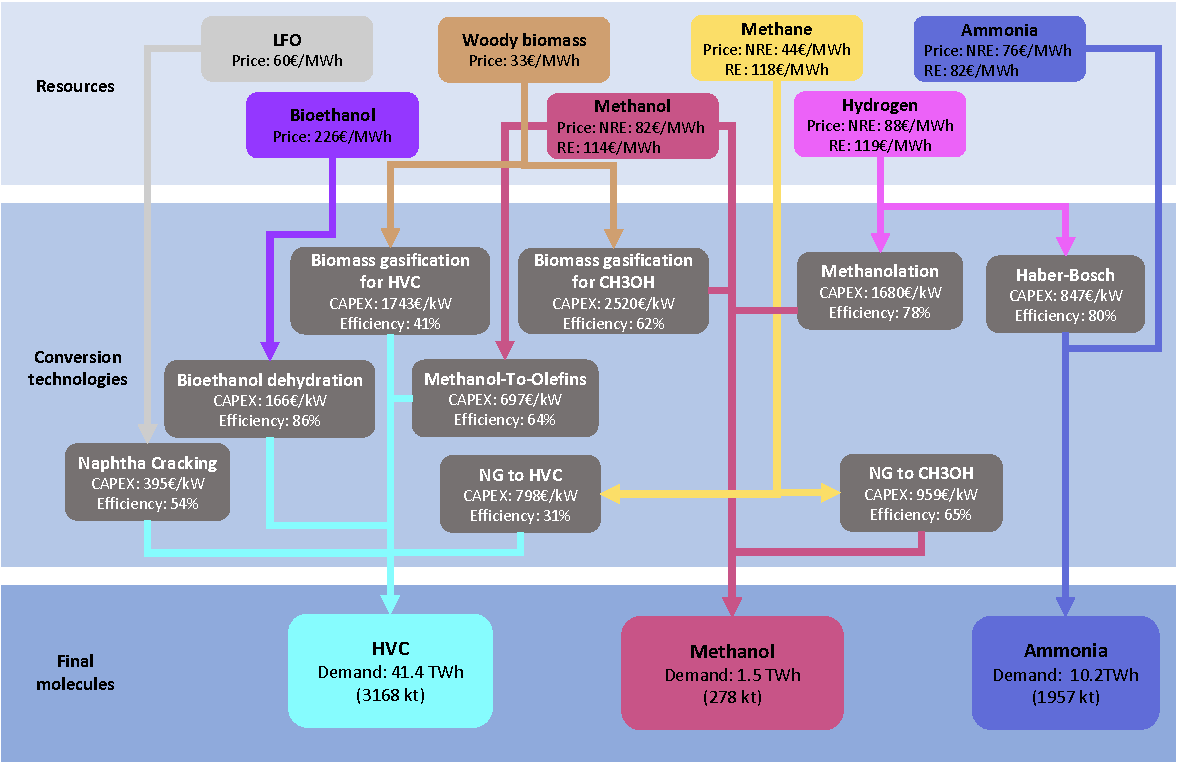
\includegraphics[width=\textwidth]{NED_tech.pdf}
\label{fig:NED_tech}
\end{figure}


\section{Chapter 4 - Reinforcement Learning}
\label{Chap_RL}


\subsection{Binding}
\label{RL_binding}

\begin{mdframed}[style=comment] % Comment from the reviewer
{\color{violet} \textbf{Christophe}} - The concept of binding constraint was not clear.
\end{mdframed}

\noindent
Besides the information given in Section 4.2.3 of the manuscript (and reminded here below), I do not see further explanations that could clarify the concept of binding constraint in a Linear Programming (LP) problem. Consequently, regarding this comment, there has not been further modification brought to the manuscript.


\begin{mdframed}[style=manuscript] % Modification brought to the manuscript
To identify the actions that have an actual impact on the environment, we can check if they are binding or not. In a LP problem, constraints represent hyperplanes in the domain of variables. In a two-dimension space, these are straight lines (see Figure \ref{fig:Binding_constr}). When the problem is bounded and feasible, these lines are the edges of a convex polygon: the domain of feasibility. The optimal solution, $\textbf{x}^*$, is the combination of variables leading to the optimal value of the objective function. Besides being within the domain of feasibility, it is proven that this optimal solution, when unique\footnote{There are cases where the objective function has the same optimal value along an entire edge. In this case, there is an infinity of solutions and the problem is indeterminate.}, locates on a vertex of the domain \cite{bertsimas1997introduction}. The constraints intersecting at this vertex are considered as binding, actually limiting the objective function to be more optimal. In other words, binding constraints, when tightened, aggravate the objective value function. If these are inequality constraints, as represented in Figure \ref{fig:Binding_constr}, it means that their left and right sides of the equation are equal.
\end{mdframed}

\begin{figure}[!htbp]
\centering
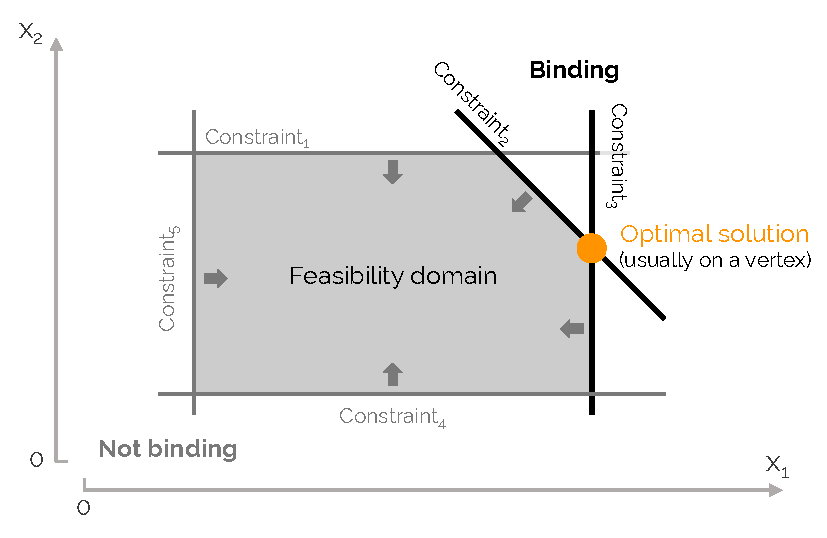
\includegraphics[width=0.7\textwidth]{Binding_constr.pdf}
\caption{Binding versus non-binding constraints. In LP where the feasibility domain is non-empty and bounded, the constraints defined a convex feasibility domain in the space of variables (here, x$_1$ and x$_2$). The optimal solution usually locates on a vertex of this domain, \ie the intersection of several constraints (here, constraints 2 and 3) limiting the solution. These constraints are considered as binding, \ie having a limiting impact on the optimal solution.}
\label{fig:Binding_constr}
\end{figure}

\section{Principal Component Analysis}
\label{PCA}

\subsection{Confusion with the word PC}
\label{Confusion_PC_wording}


\begin{mdframed}[style=comment] % Comment from the reviewer
{\color{violet} \textbf{Christophe}} When using the word ``component'', there seems to be a confusion and it is not always easy to understand if you refer to the vector or the coefficient related to one of the original variable.
\end{mdframed}

\noindent The confusion probably comes from the fact a Principal Component (PC) actually represents an eigenvector of the covariance matrix. This vector is, by definition, composed of \textbf{components}, each of them being a coefficient related to a specific original variable. Parts where the word ``component'' is not directly linked to ``vector'', ``eigenvector'' or ``PC'' are those that could mislead the reader. Modifications have been brought to these parts.

{\color{blue} End of second paragraph of section 1.4.1}:

\begin{mdframed}[style=manuscript] % Modification brought to the manuscript
Moreover, this means that \textbf{the coefficient} $\alpha_{ki}$, \ie the component of $\bm{\alpha}_{\mathbf{k}}$ related to the $i^{\text{th}}$ original variable, $x_i$,  gives its weight in the $k^{\text{th}}$ PC, \ie $z_k$. 
\end{mdframed}


\clearpage
\def\bibfont{\scriptsize}
\bibliography{../bib_thesis.bib}
\normalsize

\end{document}